\documentclass[12pt]{article}
\usepackage{hyperref}
\usepackage{graphicx}
\usepackage{parskip}
\usepackage{float}
\usepackage{amsmath}
\usepackage{amssymb}

\hypersetup{
    colorlinks,
    citecolor=black,
    filecolor=black,
    linkcolor=black,
    urlcolor=black
}

\title{PEU 356 Assignment 1}
\author{Mohamed Hussien El-Deeb (201900052)}
\date{\today}

\begin{document}

\maketitle
\tableofcontents

\section{3.10.1}

\[
    xy = u, x^2 - y^2 = v, z = z
\]

\subsection{a}

\(u\) curves are \(\frac{n}{x}\) asymptotes, \(u=0\) is xz-plane, repeated for all values of \(z\).

\[
    (x, \frac{u_i}{x}, z)
\]

\(v\) curves are x shaped for \(v=0\), horizontal hyperbola for \(v>0\), vertical hyperbola for \(v<0\), repeated for all values of \(z\).

\[
    (x, \pm\sqrt{x^2 - v_i}, z)
\]

\(z\) curves are planes parallel to xy-plane.


\[
    (x, y, z_i)
\]

\subsection{b}

\begin{figure}[H]
    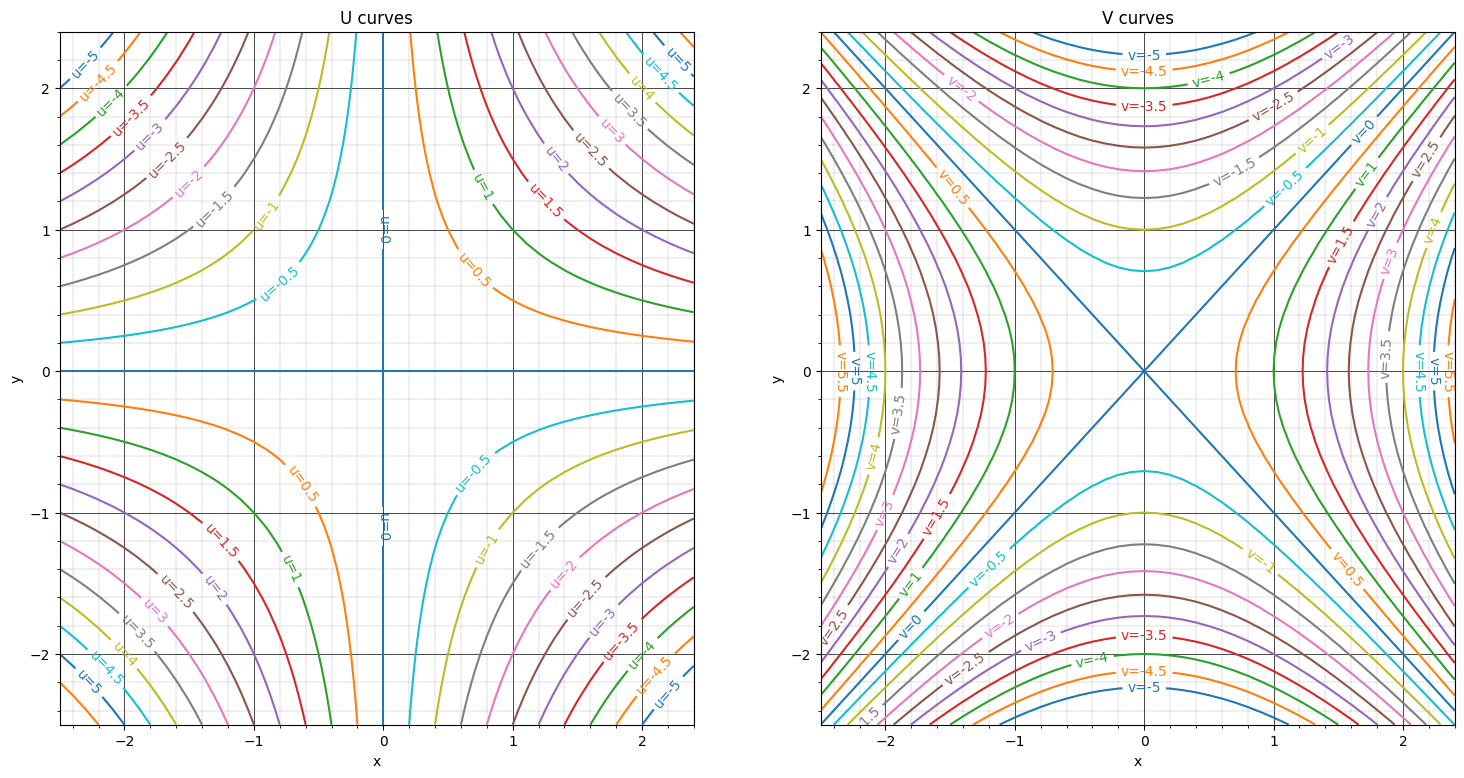
\includegraphics[width=\linewidth]{Q1B.png}
    \caption{U and V curves.}\label{fig:Q1B}
\end{figure}

\begin{figure}[H]
    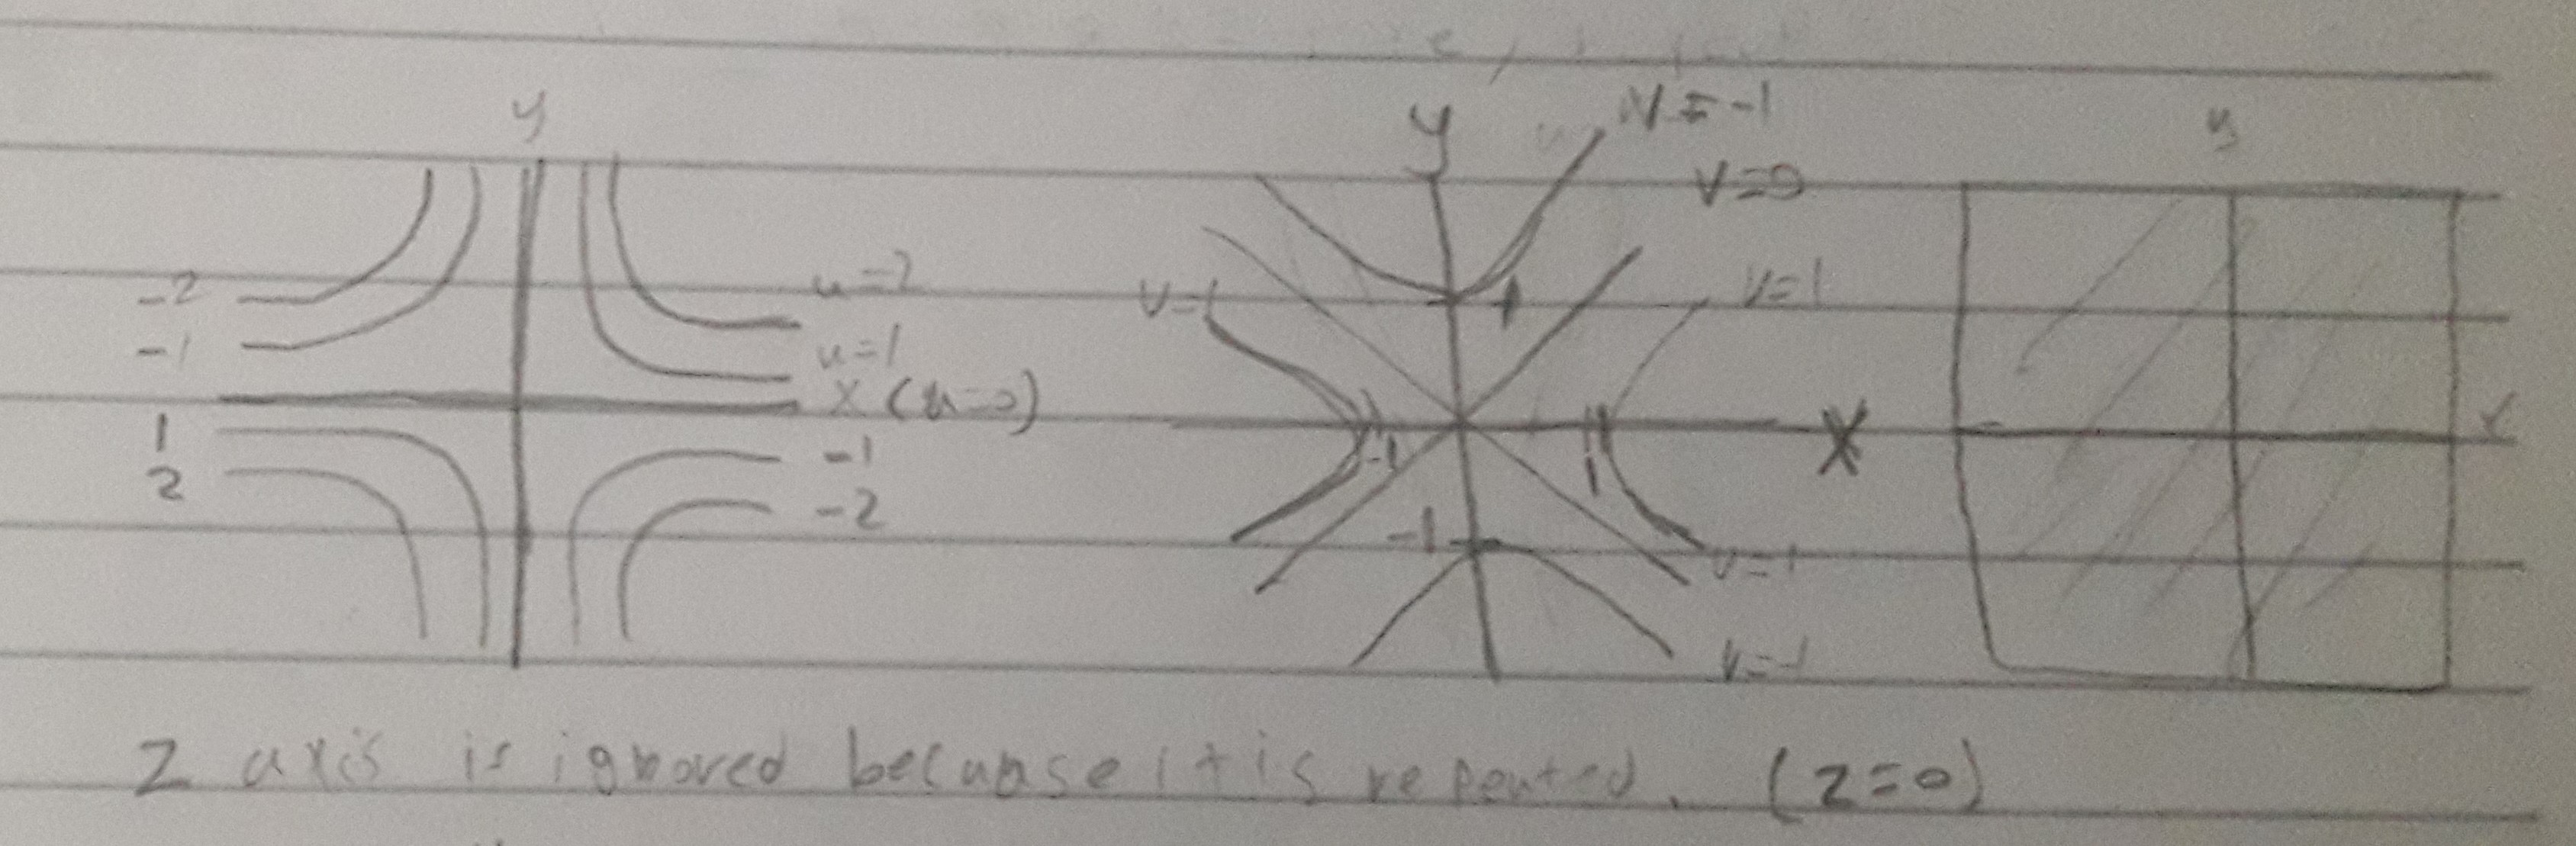
\includegraphics[width=\linewidth]{Q1B.jpg}
    \caption{U and V curves sketch.}\label{fig:Q1B2}
\end{figure}

\subsection{c}

\[
    \nabla u = \frac{ \partial u}{\partial x} \hat{\dot{\imath}}
    + \frac{ \partial u}{\partial y}  \hat{\dot{\jmath}} = \frac{ \partial (xy)}{\partial x}  \hat{\dot{\imath}}
    + \frac{ \partial (xy)}{\partial y}  \hat{\dot{\jmath}} = y  \hat{\dot{\imath}}
    + x  \hat{\dot{\jmath}}
\]

\[
    \nabla v = \frac{ \partial v}{\partial x} \hat{\dot{\imath}}
    + \frac{ \partial v}{\partial y}  \hat{\dot{\jmath}}
    = \frac{ \partial (x^2 - y^2)}{\partial x}  \hat{\dot{\imath}}
    + \frac{ \partial (x^2 - y^2)}{\partial y}  \hat{\dot{\jmath}}
    = 2x  \hat{\dot{\imath}} - 2y  \hat{\dot{\jmath}}
\]

\[
    \hat{\textbf{e}}_u = \frac{\nabla u}{|\nabla u|} = \frac{y  \hat{\dot{\imath}}
        + x  \hat{\dot{\jmath}}}{\sqrt{x^2 + y^2}}
\]

\[
    \hat{\textbf{e}}_v = \frac{\nabla v}{|\nabla v|} = \frac{2x  \hat{\dot{\imath}}
        - 2y  \hat{\dot{\jmath}}}{\sqrt{4x^2 + 4y^2}}
\]

\begin{figure}[H]
    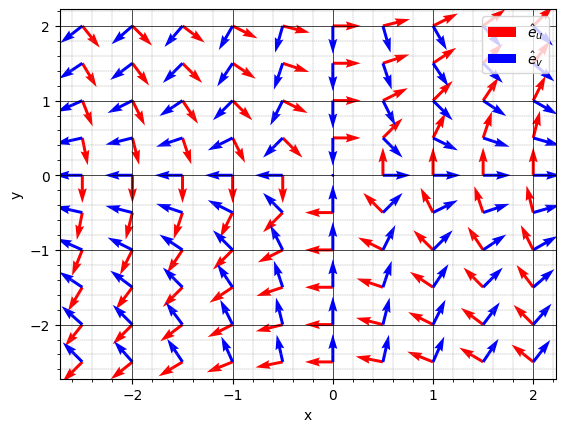
\includegraphics[width=\linewidth]{Q1C.png}
    \caption{Basis Vectors Field Plot}\label{fig:Q1C}
\end{figure}

\begin{figure}[H]
    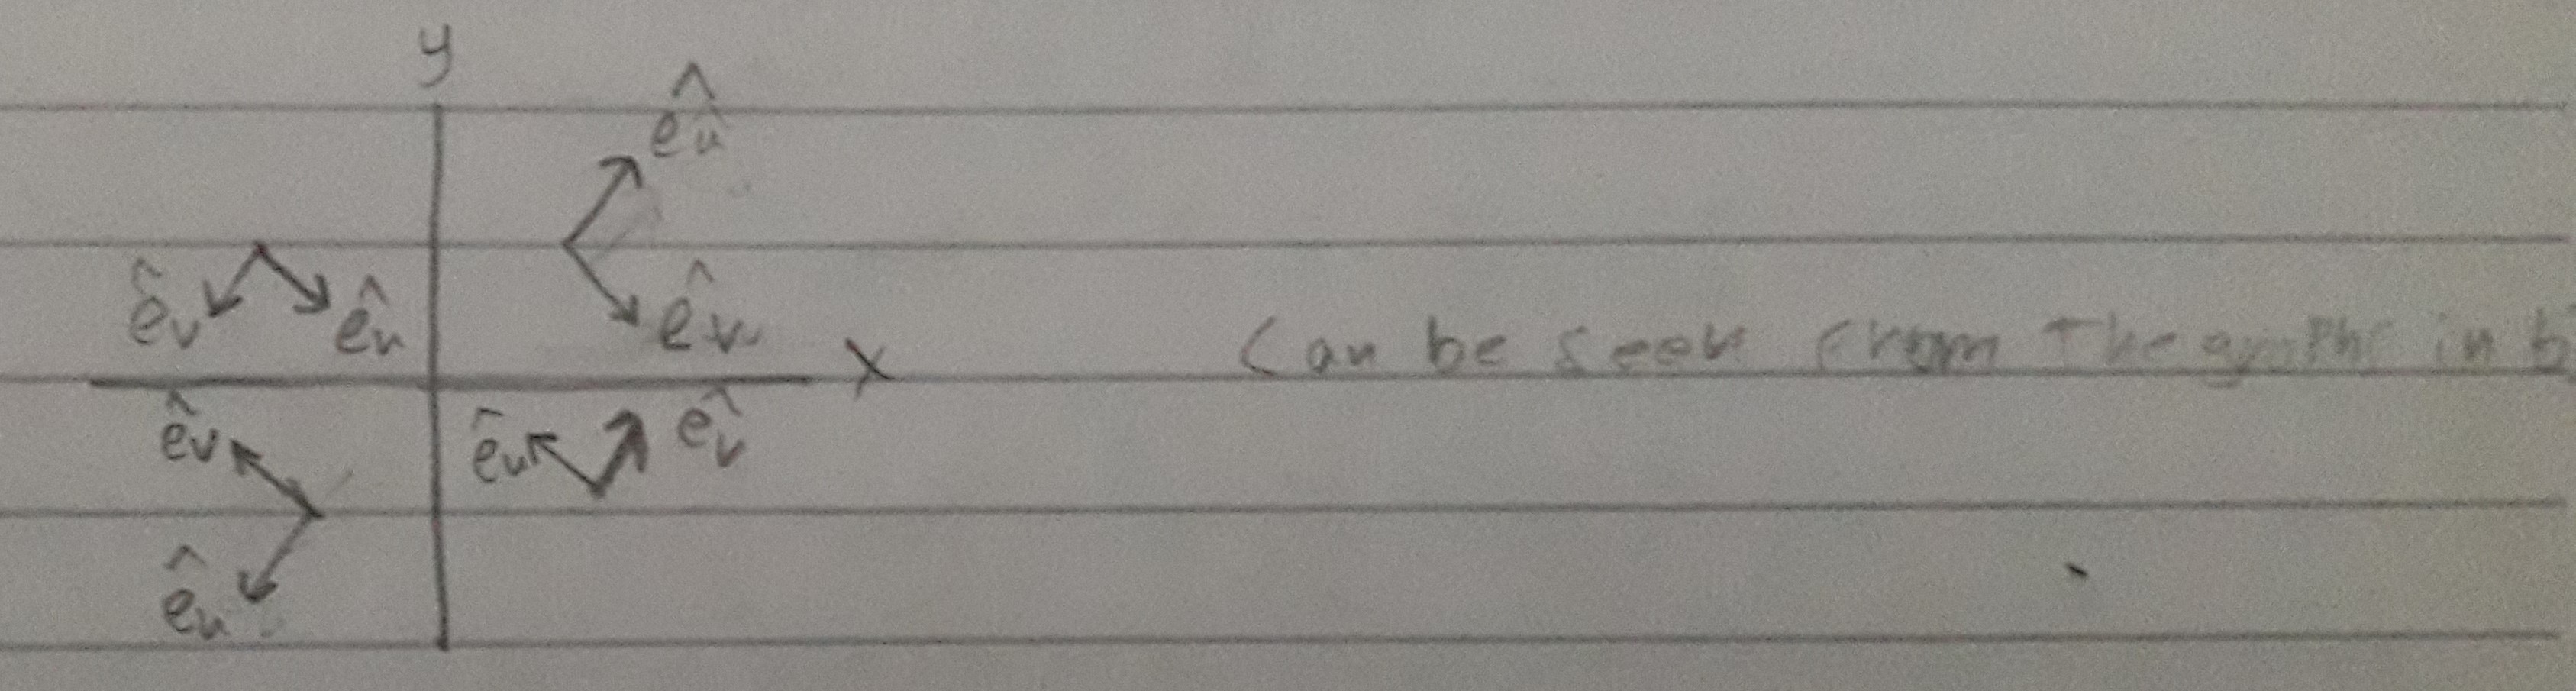
\includegraphics[width=\linewidth]{Q1C.jpg}
    \caption{Basis Vectors Field Plot sketch.}\label{fig:Q1C2}
\end{figure}

\subsection{d}

\[
    \hat{\textbf{e}}_u \times \hat{\textbf{e}}_v =
    \begin{vmatrix}
        \hat{\dot{\imath}}         & \hat{\dot{\jmath}}          & \hat{k} \\
        \frac{y}{\sqrt{x^2 + y^2}} & \frac{x}{\sqrt{x^2 + y^2}}  & 0       \\
        \frac{x}{\sqrt{x^2 + y^2}} & -\frac{y}{\sqrt{x^2 + y^2}} & 0       \\
    \end{vmatrix}
\]

\[
    = \left(
    - \frac{y}{\sqrt{x^2 + y^2}} \frac{y}{\sqrt{x^2 + y^2}}
    - \frac{x}{\sqrt{x^2 + y^2}} \frac{x}{\sqrt{x^2 + y^2}}
    \right) \hat{k} = -\hat{k}
\]

From the previous result, we can see that the coordinate system is left-handed.

\section{3.10.4}

\(\hat{\textbf{e}}_1\) is the unit vector in the direction of increasing \(q_1\).

\(\hat{\textbf{e}}_1 = \left\langle1, 0, 0\right\rangle \)

\subsection{a}

\[
    \nabla \cdot \textbf{V} = \frac{1}{h_1 h_2 h_3}
    \left[
        \frac{\partial}{\partial q_1}\left(V_1 h_2 h_3\right)
        + \frac{\partial}{\partial q_2}\left(V_2 h_1 h_3\right)
        + \frac{\partial}{\partial q_3}\left(V_3 h_1 h_2\right)
        \right]
\]

\[
    \nabla \cdot \hat{\textbf{e}}_1 = \frac{1}{h_1 h_2 h_3}
    \left[
        \frac{\partial}{\partial q_1}\left(1 * h_2 h_3\right)
        + \frac{\partial}{\partial q_2}\left(0 * h_1 h_3\right)
        + \frac{\partial}{\partial q_3}\left(0 * h_1 h_2\right)
        \right]
\]

\[
    \nabla \cdot \hat{\textbf{e}}_1 = \frac{1}{h_1 h_2 h_3} \frac{\partial}{\partial q_1}\left(h_2 h_3\right)
\]

\subsection{b}

\[
    \nabla \times \textbf{V} = \frac{1}{h_1 h_2 h_3}
    \begin{vmatrix}
        \hat{\textbf{e}}_1 h_1        & \hat{\textbf{e}}_2 h_2        & \hat{\textbf{e}}_3 h_3        \\
        \frac{\partial}{\partial q_1} & \frac{\partial}{\partial q_2} & \frac{\partial}{\partial q_3} \\
        h_1 V_1                       & h_2 V_2                       & h_3 V_3                       \\
    \end{vmatrix}
\]

\[
    \nabla \times \hat{\textbf{e}}_1 = \frac{1}{h_1 h_2 h_3}
    \begin{vmatrix}
        \hat{\textbf{e}}_1 h_1        & \hat{\textbf{e}}_2 h_2        & \hat{\textbf{e}}_3 h_3        \\
        \frac{\partial}{\partial q_1} & \frac{\partial}{\partial q_2} & \frac{\partial}{\partial q_3} \\
        h_1*1                         & h_2*0                         & h_3*0                         \\
    \end{vmatrix}
\]

\[
    \nabla \times \hat{\textbf{e}}_1 = \frac{1}{h_1 h_2 h_3}
    \left(
    \hat{\textbf{e}}_2 h_2 \frac{\partial h_1}{\partial q_3}
    - \hat{\textbf{e}}_3 h_3 \frac{\partial h_1}{\partial q_2}
    \right)
\]

\[
    \nabla \times \hat{\textbf{e}}_1 = \frac{1}{h_1}
    \left[
        \hat{\textbf{e}}_2 \frac{1}{h_3} \frac{\partial h_1}{\partial q_3}
        - \hat{\textbf{e}}_3  \frac{1}{h_2}  \frac{\partial h_1}{\partial q_2}
        \right]
\]

\section{3.10.5}

\[
    \hat{\textbf{e}}_i = \frac{1}{h_i} \frac{\partial \textbf{r}}{\partial q_i}
\]

\[
    \hat{\textbf{e}}_i \cdot \hat{\textbf{e}}_j = \frac{1}{h_i h_j}
    \left(\frac{\partial \textbf{r}}{\partial q_i}\right)
    \cdot \left(\frac{\partial \textbf{r}}{\partial q_j}\right)  = \delta_{ij}
\]

\[
    \frac{\partial \textbf{r}}{\partial q_i} = \frac{\partial (x_j \hat{\varepsilon}_j)}{\partial q_i}
    = \frac{\partial x_j}{\partial q_i} \hat{\varepsilon}_j + x_j \frac{\partial \hat{\varepsilon}_j}{\partial q_i}
\]

\[
    \because  \hat{\varepsilon}_{ij} = \delta_{ij}
\]

\[
    \therefore \frac{\partial \hat{\varepsilon}_j}{\partial q_i} = 0
\]

\[
    \frac{\partial \textbf{r}}{\partial q_i} = \frac{\partial x_j}{\partial q_i} \hat{\varepsilon}_j
\]

\[
    \frac{\partial \textbf{r}}{\partial q_i} \cdot \frac{\partial \textbf{r}}{\partial q_j}
    = \frac{\partial x_k}{\partial q_i} \frac{\partial x_m}{\partial q_j}
    \left(\hat{\varepsilon}_k \cdot \hat{\varepsilon}_m\right)
\]

\[
    = \frac{\partial x_k}{\partial q_i} \frac{\partial x_m}{\partial q_j} \delta_{km}
    = \frac{\partial x_k}{\partial q_i} \frac{\partial x_k}{\partial q_j}
\]

\[
    \hat{\textbf{e}}_i \cdot \hat{\textbf{e}}_j
    = \frac{1}{h_i h_j} \frac{\partial x_k}{\partial q_i} \frac{\partial x_k}{\partial q_j} = \delta_{ij}
\]

\[
    \frac{\partial x_k}{\partial q_i} \frac{\partial x_k}{\partial q_j} = h_i h_j \delta_{ij}
\]

\[
    i = j \implies {\left(\frac{\partial x_k}{\partial q_i}\right)}^2 = h_i^2
\]

\[
    \frac{\partial \hat{\textbf{e}}_i}{\partial q_j} = \frac{\partial}{\partial q_j}
    \left(\frac{1}{h_i} \frac{\partial \textbf{r}}{\partial q_i}\right)
    = \frac{\partial}{\partial q_j} \left(\frac{1}{h_i} \frac{\partial x_k}{\partial q_i} \hat{\varepsilon}_k\right)
\]

\[
    = \frac{\partial}{\partial q_j} \left(\frac{1}{h_i} \frac{\partial x_k}{\partial q_i}\right) \hat{\varepsilon}_k
\]

\[
    = \frac{1}{h_i}
    \left(
    \frac{\partial^2 x_k}{\partial q_j \partial q_i}
    - \frac{1}{h_i} \frac{\partial h_i}{\partial q_j} \frac{\partial x_k}{\partial q_i}
    \right) \hat{\varepsilon}_k
\] % TODO: finish this

\section{3.10.28}

\[
    x = r \sin{\theta} \cos{\varphi}, y = r \sin{\theta} \sin{\varphi}, z = r \cos{\theta}
\]

\[
    \nabla = \hat{\textbf{e}}_1 \frac{1}{h_1} \frac{\partial}{\partial q_1}
    + \hat{\textbf{e}}_2 \frac{1}{h_2} \frac{\partial}{\partial q_2}
    + \hat{\textbf{e}}_3 \frac{1}{h_3} \frac{\partial}{\partial q_3}
\]

\[
    \nabla_{xyz} =  \hat{\dot{\imath}} \frac{\partial}{\partial x}
    + \hat{\dot{\jmath}} \frac{\partial}{\partial y}
    +  \hat{k} \frac{\partial}{\partial z}
\]

\[
    \nabla_{r \theta \varphi } = \hat{\textbf{e}}_r \frac{\partial}{\partial r}
    + \hat{\textbf{e}}_\theta \frac{1}{r} \frac{\partial}{\partial \theta}
    + \hat{\textbf{e}}_\varphi \frac{1}{r \sin{\theta}} \frac{\partial}{\partial \varphi}
\]

\[
    \nabla_{xyz} = \nabla_{r \theta \varphi }
\]

\[
    \hat{\dot{\imath}} \frac{\partial}{\partial x}
    + \hat{\dot{\jmath}} \frac{\partial}{\partial y}
    +  \hat{k} \frac{\partial}{\partial z} = \hat{\textbf{e}}_r \frac{\partial}{\partial r}
    + \hat{\textbf{e}}_\theta \frac{1}{r} \frac{\partial}{\partial \theta}
    + \hat{\textbf{e}}_\varphi \frac{1}{r \sin{\theta}} \frac{\partial}{\partial \varphi}
\]

\[
    \hat{\textbf{e}}_r = \frac{\partial x_j}{\partial r} \hat{\varepsilon}_j
    + x_j \frac{\partial \hat{\varepsilon}_j}{\partial r} = \frac{\partial x}{\partial r} \hat{\dot{\imath}}
    + \frac{\partial y}{\partial r} \hat{\dot{\jmath}} + \frac{\partial z}{\partial r} \hat{k}
\]

\[
    = \sin{\theta} \cos{\varphi} \hat{\dot{\imath}} + \sin{\theta} \sin{\varphi} \hat{\dot{\jmath}}
    + \cos{\theta} \hat{k}
\]

\[
    \hat{\textbf{e}}_\theta = \cos{\theta} \cos{\varphi} \hat{\dot{\imath}}
    + \cos{\theta} \sin{\varphi} \hat{\dot{\jmath}} - \sin{\theta} \hat{k}
\]

\[
    \hat{\textbf{e}}_\varphi = -\sin{\varphi} \hat{\dot{\imath}} + \cos{\varphi} \hat{\dot{\jmath}}
\]

\[
    \hat{\dot{\imath}} \frac{\partial}{\partial x} + \hat{\dot{\jmath}} \frac{\partial}{\partial y}
    +  \hat{k} \frac{\partial}{\partial z} =
    \left(
    \sin{\theta} \cos{\varphi} \hat{\dot{\imath}}
    + \sin{\theta} \sin{\varphi} \hat{\dot{\jmath}}
    + \cos{\theta} \hat{k}
    \right)  \frac{\partial}{\partial r}
\]

\[
    + \left(
    \cos{\theta} \cos{\varphi} \hat{\dot{\imath}} + \cos{\theta} \sin{\varphi} \hat{\dot{\jmath}}
    - \sin{\theta} \hat{k}
    \right) \frac{1}{r} \frac{\partial}{\partial \theta}
\]

\[
    + \left(-\sin{\varphi} \hat{\dot{\imath}} + \cos{\varphi} \hat{\dot{\jmath}}\right)
    \frac{1}{r \sin{\theta}} \frac{\partial}{\partial \varphi}
\]

\[
    = \hat{\dot{\imath}}
    \left(
    \sin{\theta} \cos{\varphi} \frac{\partial}{\partial r}
    + \cos{\theta} \cos{\varphi} \frac{1}{r} \frac{\partial}{\partial \theta}
    - \sin{\varphi} \frac{1}{r \sin{\theta}} \frac{\partial}{\partial \varphi}
    \right)
\]

\[
    + \hat{\dot{\jmath}}
    \left(
    \sin{\theta} \sin{\varphi} \frac{\partial}{\partial r}
    + \cos{\theta} \sin{\varphi} \frac{1}{r} \frac{\partial}{\partial \theta}
    + \cos{\varphi} \frac{1}{r \sin{\theta}} \frac{\partial}{\partial \varphi}
    \right)
\]

\[
    + \hat{k} \left(\cos{\theta} \frac{\partial}{\partial r}
    - \sin{\theta} \frac{1}{r} \frac{\partial}{\partial \theta} \right)
\]

\[
    \frac{\partial}{\partial x} = \sin{\theta} \cos{\varphi} \frac{\partial}{\partial r}
    + \cos{\theta} \cos{\varphi} \frac{1}{r} \frac{\partial}{\partial \theta}
    - \sin{\varphi} \frac{1}{r \sin{\theta}} \frac{\partial}{\partial \varphi}
\]

\[
    \frac{\partial}{\partial y} = \sin{\theta} \sin{\varphi} \frac{\partial}{\partial r}
    + \cos{\theta} \sin{\varphi} \frac{1}{r} \frac{\partial}{\partial \theta}
    + \cos{\varphi} \frac{1}{r \sin{\theta}} \frac{\partial}{\partial \varphi}
\]

\[
    \frac{\partial}{\partial z} = \cos{\theta} \frac{\partial}{\partial r}
    - \sin{\theta} \frac{1}{r} \frac{\partial}{\partial \theta}
\]

\section{3.10.29}

\[
    x = r \sin{\theta} \cos{\varphi}, y = r \sin{\theta} \sin{\varphi}
\]

\[
    -i \left(x \frac{\partial}{\partial y} - y \frac{\partial}{\partial x}\right)
\]

\[
    =
    -i r \sin{\theta} \cos{\varphi}
    \left(
    \sin{\theta} \sin{\varphi} \frac{\partial}{\partial r}
    + \cos{\theta} \sin{\varphi} \frac{1}{r} \frac{\partial}{\partial \theta}
    + \cos{\varphi} \frac{1}{r \sin{\theta}} \frac{\partial}{\partial \varphi}
    \right)
\]

\[
    + i r \sin{\theta} \sin{\varphi}
    \left(
    \sin{\theta} \cos{\varphi} \frac{\partial}{\partial r}
    + \cos{\theta} \cos{\varphi} \frac{1}{r} \frac{\partial}{\partial \theta}
    - \sin{\varphi} \frac{1}{r \sin{\theta}} \frac{\partial}{\partial \varphi}
    \right)
\]

\[
    = i r \sin{\theta}
    \left(\sin{\theta} \sin{\varphi} \cos{\varphi} - \sin{\theta} \sin{\varphi} \cos{\varphi} \right)
    \frac{\partial}{\partial r}
\]

\[
    + i r \sin{\theta}
    \left(\sin{\varphi} \cos{\varphi} - \sin{\varphi} \cos{\varphi}\right)
    \cos{\theta} \frac{1}{r} \frac{\partial}{\partial \theta}
\]

\[
    - i \left(\sin^2{\varphi} + \cos^2{\varphi} \right) \frac{\partial}{\partial \varphi}
\]

\[
    = - i \frac{\partial}{\partial \varphi}
\]

\section{3.10.30}

\[
    L = -i \left(\textbf{r} \times \nabla\right)
\]

\[
    = -i \left\lvert \begin{array}{ccc}
        \hat{\dot{\imath}}          & \hat{\dot{\jmath}}          & \hat{k}                     \\
        x                           & y                           & z                           \\
        \frac{\partial}{\partial x} & \frac{\partial}{\partial y} & \frac{\partial}{\partial z} \\
    \end{array} \right\rvert
\]

\[
    =
    -i
    \left(
    \hat{\dot{\imath}} \left(y \frac{\partial}{\partial z} - z \frac{\partial}{\partial y}\right)
    + \hat{\dot{\jmath}} \left(z \frac{\partial}{\partial x} - x \frac{\partial}{\partial z}\right)
    + \hat{k} \left(x \frac{\partial}{\partial y} - y \frac{\partial}{\partial x}\right)
    \right)
\]

\[
    = i \left(z \frac{\partial}{\partial y} - y \frac{\partial}{\partial z}\right) \hat{\dot{\imath}}
    + i \left(x \frac{\partial}{\partial z} - z \frac{\partial}{\partial x}\right) \hat{\dot{\jmath}}
    + i \left(y \frac{\partial}{\partial x} - x \frac{\partial}{\partial y}\right) \hat{k}
\]

\[
    L_x = i \left(z \frac{\partial}{\partial y} - y \frac{\partial}{\partial z}\right)
\]

\[
    L_y = i \left(x \frac{\partial}{\partial z} - z \frac{\partial}{\partial x}\right)
\]

\[
    L_z = i \left(y \frac{\partial}{\partial x} - x \frac{\partial}{\partial y}\right)
\]

\subsection{a}

\[
    L_x
    + i L_y = i \left(z \frac{\partial}{\partial y} - y \frac{\partial}{\partial z}\right)
    - \left(x \frac{\partial}{\partial z} - z \frac{\partial}{\partial x}\right)
\]

\[
    = z \frac{\partial}{\partial x} + i z \frac{\partial}{\partial y} - \left(x + i y\right)  \frac{\partial}{\partial z}
\]

\[
    = z \left(\frac{\partial}{\partial x} + i \frac{\partial}{\partial y}\right)  - \left(x + i y\right)
    \frac{\partial}{\partial z}
\]

\[
    x + i y = r \sin{\theta} \cos{\varphi} + i r \sin{\theta} \sin{\varphi} = r \sin{\theta}
    \left(\cos{\varphi} + i \sin{\varphi}\right) = r \sin{\theta} e^{i \varphi}
\]

\[
    \frac{\partial}{\partial x} + i \frac{\partial}{\partial y} =
\]

\[
    \sin{\theta} \cos{\varphi} \frac{\partial}{\partial r}
    + \cos{\theta} \cos{\varphi} \frac{1}{r} \frac{\partial}{\partial \theta}
    - \sin{\varphi} \frac{1}{r \sin{\theta}} \frac{\partial}{\partial \varphi}
\]

\[
    + i  \sin{\theta} \sin{\varphi} \frac{\partial}{\partial r}
    + i \cos{\theta} \sin{\varphi} \frac{1}{r} \frac{\partial}{\partial \theta}
    + i \cos{\varphi} \frac{1}{r \sin{\theta}} \frac{\partial}{\partial \varphi}
\]

\[
    = \sin{\theta} \left(\cos{\varphi} + i \sin{\varphi}\right) \frac{\partial}{\partial r}
    + \cos{\theta} \left(\cos{\varphi} + i \sin{\varphi}\right) \frac{1}{r} \frac{\partial}{\partial \theta}
\]

\[
    + \left(i \cos{\varphi} - \sin{\varphi}\right)  \frac{1}{r \sin{\theta}} \frac{\partial}{\partial \varphi}
\]

\[
    = e^{i \varphi}
    \left(
    \sin{\theta} \frac{\partial}{\partial r}+ \cos{\theta} \frac{1}{r} \frac{\partial}{\partial \theta}
    + i \frac{1}{r \sin{\theta}} \frac{\partial}{\partial \varphi}
    \right)
\]

\[
    L_x + i L_y =
\]

\[
    r \cos{\theta} e^{i \varphi}
    \left(
    \sin{\theta} \frac{\partial}{\partial r}
    + \cos{\theta} \frac{1}{r} \frac{\partial}{\partial \theta}
    + i \frac{1}{r \sin{\theta}} \frac{\partial}{\partial \varphi}
    \right)
\]

\[
    - r \sin{\theta} e^{i \varphi}
    \left(\cos{\theta} \frac{\partial}{\partial r} - \sin{\theta} \frac{1}{r} \frac{\partial}{\partial \theta}\right)
\]

\[
    = r e^{i \varphi}
    \left(
    \sin{\theta} \cos{\theta} \frac{\partial}{\partial r}
    + \frac{\cos^2{\theta}}{r} \frac{\partial}{\partial \theta}
    + i \cot{\theta} \frac{1}{r}\frac{\partial}{\partial \varphi}
    - \sin{\theta} \cos{\theta} \frac{\partial}{\partial r}
    + \frac{\sin^2{\theta}}{r} \frac{\partial}{\partial \theta}
    \right)
\]

\[
    = e^{i \varphi}
    \left(
    \frac{\partial}{\partial \theta}
    + i \cot{\theta}\frac{\partial}{\partial \varphi}
    \right)
\]

\subsection{b}

\[
    L_x - i L_y = i \left(z \frac{\partial}{\partial y} - y \frac{\partial}{\partial z}\right)
    + \left(x \frac{\partial}{\partial z} - z \frac{\partial}{\partial x}\right)
\]

\[
    = z \left(i \frac{\partial}{\partial y} - \frac{\partial}{\partial x}\right) + \left( x - i y\right)
    \frac{\partial}{\partial z}
\]

\[
    x - i y = r \sin{\theta} \cos{\varphi} - i r \sin{\theta} \sin{\varphi} = r \sin{\theta}
    \left(\cos{\varphi} - i \sin{\varphi}\right) = r \sin{\theta} e^{-i \varphi}
\]

\[
    i \frac{\partial}{\partial y} - \frac{\partial}{\partial x} =
\]

\[
    i  \sin{\theta} \sin{\varphi} \frac{\partial}{\partial r}
    + i \cos{\theta} \sin{\varphi} \frac{1}{r} \frac{\partial}{\partial \theta}
    + i \cos{\varphi} \frac{1}{r \sin{\theta}} \frac{\partial}{\partial \varphi}
\]

\[
    - \sin{\theta} \cos{\varphi} \frac{\partial}{\partial r}
    - \cos{\theta} \cos{\varphi} \frac{1}{r} \frac{\partial}{\partial \theta}
    + \sin{\varphi} \frac{1}{r \sin{\theta}} \frac{\partial}{\partial \varphi}
\]

\[
    = \sin{\theta} \left(\cos{\varphi} - i \sin{\varphi}\right)
    \frac{\partial}{\partial r} + \cos{\theta} \left(\cos{\varphi} - i \sin{\varphi}\right)
    \frac{1}{r} \frac{\partial}{\partial \theta}
\]

\[
    + \left(i \cos{\varphi} + \sin{\varphi}\right) \frac{1}{r \sin{\theta}} \frac{\partial}{\partial \varphi}
\]

\[
    = e^{-i \varphi}
    \left(
    \sin{\theta} \frac{\partial}{\partial r} + \cos{\theta} \frac{1}{r} \frac{\partial}{\partial \theta}
    + i \frac{1}{r \sin{\theta}} \frac{\partial}{\partial \varphi}
    \right)
\]

\section{3.10.31}

\section{3.10.32}

\subsection{a}

\subsection{b}

\subsection{c}

\end{document}